\documentclass[12pt,letterpaper,boxed]{hmcpset}
\usepackage[margin=1in,headheight=14pt]{geometry}
\usepackage{amsfonts, amsmath, amssymb, enumerate, fancyhdr, gensymb, lastpage, mathtools, parskip, graphicx}
\usepackage{xcolor, tikz-cd}
\newcommand{\wg}[1]{\textcolor{violet}{#1}}
\newcommand{\OO}{\mathcal O}
\newcommand{\Q}{\mathbb Q}
\newcommand{\R}{\mathbb R}
\newcommand{\C}{\mathcal C}
\newcommand{\Z}{\mathbb Z}
\newcommand{\abs}[1]{\left|#1\right|}
\newcommand{\im}{\text{im }}
\newcommand{\inv}{^{-1}}
\newcommand{\normal}{\unlhd} %% one can also use \trianglelelefteq
\newcommand{\anglee}[1]{\langle #1 \rangle}
\usepackage[shortlabels]{enumitem}

% Numbering macros
\pagestyle{fancy}
\lhead{Will Gilroy}
\chead{Algebra Homework \#3}
\rhead{30 Sept 2025}
\lfoot{}
\cfoot{}
\rfoot{Page\ \thepage\ of\ \pageref{LastPage}}

\linespread{1.5}

\newcommand\blankpage{
    \thispagestyle{empty}
    \addtocounter{page}{-1}
    \newpage}
\renewcommand\footrulewidth{0.4pt}

\begin{document}

\problemlist{Algebra Homework \#3} 

%------------------------- Problem 1 -----------------------

\begin{problem}
	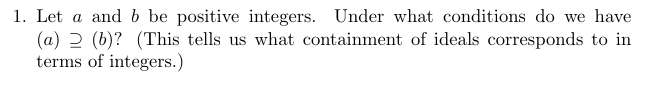
\includegraphics[scale=0.8]{1.png}
	\hfill
\end{problem}

\begin{solution}
Although we are working with integers, note that in any ring $R$ with
$1\neq 0$ we have $a = \sum_{i=1}^a 1 \in R$ and $b = \sum_{i=1}^b 1
\in R$ and so the following statements hold for any ring with $1 \neq
0$. 

We have $(b) \subseteq (a)$ if and only if $b \in (a)$ or $b = c\cdot
a$ for some $c \in R$. Now, since both $a,b$ are positive multiples of $1$ we
have that $c \in \Z_+$. In other words, $a$ divides $b$. This tells us
that containment of such ideals is ``relation reversing'' compared with
divisibility of integers.
\end{solution}

\newpage

%------------------------- Problem 2 -----------------------

\begin{problem}
	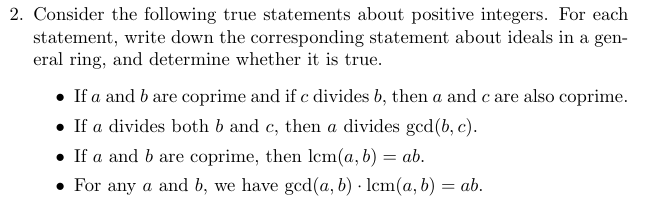
\includegraphics[scale=0.8]{2.png}
	\hfill
\end{problem}

\begin{solution}
\begin{itemize}
\item $a,b$ coprime means $gcd(a,b) = 1$. For the principal ideal
domain $R = \Z$ we have that $(a,b) = (gcd(a,b))$. And so the
corresponding statement for a general ring is:
if $(a,b) = (1) = R$ and if $(b) \subseteq (c)$ then $(a,c) = (1)$. 
Note that a ring does not necessarily have a well-defined notion of a
greatest common divisor of two elements, but it does if the ring also
happens to be a UFD. Nevertheless, let us work with the statement
above.

This statement is true. The condition $(a,b) = (1)$ means that there
exists elements $r_1, r_2 \in R$ such that $r_1a + r_2b = 1$, by
definition of ideal generated by a set. Moreover, $(b) \subseteq (c)$
means there exists some $r_3 \in R$ such that $b = r_3 c$. Combining
these statements we have \[
	1 = r_1a + r_2 b = r_1 a + r_2r_3 c \in (a,c). 
\]
In other words, indeed, $(a,c) = 1$. 

\item Recall the discussion in question $1$. The corresponding general
statement is: if $(b) \subseteq (a)$ and if $(c) \subseteq (a)$ then
$(b,c) \subseteq (a)$. 

This statement is again true. The hypothesis gives that there are
elements $r_1, r_2 \in R$ such that $b = r_1a$ and $c = r_2 a$. By
definition, a general element of $(b,c)$ is of the form $x_1 b + x_2
c$ for $x_1, x_2 \in R$. We have
\[
	x_1 b + x_2 c = x_1r_1 a + x_2r_2 a = (x_1 r_1 + x_2r_2) a \in (a). 
\]
Hence, indeed, we have $(b,c) \subseteq (a)$. 

\item The corresponding general statement is: ``if $(a,b) = (1)$ then
$(a) \cap (b) = (ab)$''. This statement is again true.

The hypothesis means that there are elements $r_1, r_2 \in R$ such
that $r_1 a + r_2 b = 1$. We show that $(a) \cap (b) = (ab)$. The
reverse inclusion is generally true since $ab = a \cdot b = b \cdot a$
and so $ab \in (a) \cap (b)$, becuase our rings are commutative.

Now we show the forward inclusion $(a) \cap (b) \subseteq (ab)$. Let
$ca \in (a) \cap (b)$. By definition, there exists some $d \in R$ such
that $db = ca$. Consider the following
\begin{align*}
	ca - db &= 0 \\
	r_2ca - d(r_2)b &= 0 \\
	r_2ca - d(1 - r_1a) &= 0 && \text{By our hypothesis} \\
	(r_2c + dr_1)a &= d \\
	(r_2c + dr_1)ab &= db \\
	(r_2c + dr_1)ab &= ra,
\end{align*}
That is we have found $ra = Kab$ for some $K \in R$ and so $ra \in
(ab)$. Hence we have $(a) \cap (b) \subseteq (ab)$ and moreso $(a)
\cap (b) = (ab)$.

\item \wg{Note to self: finish this part one day.}

\end{itemize}
\end{solution}

\newpage

%------------------------- Problem 3 -----------------------

\begin{problem}
	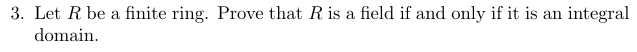
\includegraphics[scale=0.8]{3.png}
	\hfill
\end{problem}
\begin{solution}
In general we have that $R$ a field implies $R$ is an integral domain,
even if $R$ is not finite. We recount the proof here.
Suppose $R$ is a field, that is $R$ is commutative with $1 \neq 0$ and
every $a \in R$ is a two-sided unit. Now suppose we have $ab = 0$.
If $a = 0$ then we are done, so suppose 
$a$ is non-zero in
$R$. Then, $a$ has a two-sided inverse $a\inv \in R$, and so \[
	0 = ab = a\inv a b = 1 \cdot b = b.
\]
If we instead assume $b \neq 0$ then 
an extremely similar calculation will show that $ab = 0$ implies $a =
0$. \wg{(Or, perhaps it's enough that $R$ is commutative at this
point?)} 
Thus, $R$ is an integral domain.

Now suppose $R$ is finite and is an integral domain. That is, $R$ is a
commutative ring with $1 \neq 0$ and for all $a,b \in R$ we have $ab =
0$ implies $a = 0$ or $b = 0$. We show that every non-zero element in
$R$ has a two-sided inverse.
Let $a \in R$ be some non-zero element and let $\phi_a: R \to R$ be
the map defined by $\phi(r) = a\cdot r$. 

We claim that $\phi_a$ is
injective. Suppose we have $\phi(b) = \phi(c)$ for some $b,c \in R$.
That is, $ab = ac$, equivalently $a(b-c)= 0$. But recall that $a$ is a
non-zero element in the integral domain $R$, and so we must have $b-c = 0$. In
other words $b = c$ and $\phi_a$ is injective by definition.

In addition, since $R$ is finite and $\# R = \# R$, we have that
$\phi_a$ is actually a bijection. And so there must exist some $c \in
R$ such that $\phi(c) = 1$. That is, we have $c \in R$ such that $a c
= 1$. Since $R$ is commutative, $a$ is actually a two-sided unit with
inverse $c$. Thus, $R$ is a field.

\wg{Note to self: Aluffi claims that finite division rings turn out to
always be commutative. Have a read of this later if we get time}
\end{solution}

\newpage

%------------------------- Problem 4 -----------------------

\begin{problem}
	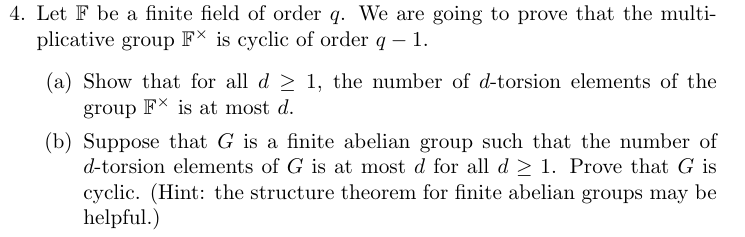
\includegraphics[scale=0.8]{4.png}
	\hfill
\end{problem}

\begin{solution}

\begin{enumerate}[(a)]
\item Consider the polynomial $f(x) = x^n - 1 \in \mathbb F[x]$. 
Recall that $\mathbb F[x]$ is a unique factorization domain
\wg{we should probably understand this better}, and so $f$ has at most
$n$ roots in $\mathbb F$. That is, there are at most $n$ elements in
$\mathbb F$ such that $a^n = 1$. And, in particular, the zero element
in the ring $\mathbb F$ does not satisfy the above equation. And so,
by the pigeonhole principle, 
all roots of $f$ must in fact lie in $\mathbb F^\times$. 
Then, recalling that an element in a group $g \in G$ is a $d$-torsion
element of $G$ if $\abs g \,\vert \, d$, the above shows that $\mathbb
F^\times$ has at most $d$ elements with $d$-torsion, for each $d \geq
1$. 
\wg{question: does $d$-torsion mean that $\abs g = d$ or that $\abs g \vert d$?}


\item I'm not sure we've super talked about the structure theorem of
finite abelian groups much, so I will recall the theorem in detail
here. \textit{Theorem:} If $G$ is a finite abelian group then we have
that $G$ is a product of cyclic groups, in particular
\[
	G \cong \Z / d_1 \Z \oplus \cdots \oplus \Z /d_s \Z,
\]
for $d_i > 0$ integers and where $d_1 \, \vert \, d_2 \vert \cdots \vert
d_n$ \wg{ew, i hate the spacing on this}. Moreover, $\abs G = d_1
\cdots d_s$. Here, we are treating $G$
as a group under addition. 

Now suppose $G$ is a finite abelian group such that the number of
$d$-torsion elements is at most $d$ for all $d \geq 1$. We show that
$s = 1$ and so $G$ is cyclic. Suppose, for contradiction,
that $s > 1$ and let $g \in G$.
We have that $\anglee g \leq G$ and so, by Lagrange's theorem, we have
that $\abs g \vert \abs G = d_1 \cdots d_s$. And so $\abs g$ divides
one of $d_i$. If $\anglee g$ divides $d_i$ then, since in particular
$d_i \vert d_s$, we also have $\anglee g \vert d_s$.
Indeed, we have $m_1 \abs g = d_i$ and $m_2 d_i = d_s$ then $m_1m_2
\abs g = d_s$, i.e., $\abs g \vert d_s$. That is $g$ is a
$d_s$-torsion element.

We have shown that all elements $g \in G$ have $d_s$-torsion.
However, we have $\abs G = d_1 \cdots d_s > d_s$. And
so we have found more than $d_s$ elements of $G$ which have
$d_s$-torsion, a contradiction. That is, we must in fact have $s=1$
and $G \cong
\Z/d\Z$ for some $d \in \mathbb N$. In other words, $G$ is a cyclic
group.


\end{enumerate}
\end{solution}

\newpage
%------------------------- Problem 5 -----------------------

\begin{problem}
	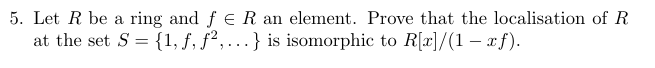
\includegraphics[scale=0.8]{5.png}
	\hfill
\end{problem}

\begin{solution}
Let us first define a map into $R[x]$: $\phi: S\inv R \to R[x]/(1-fx)$ by 
$\varphi(1/f) = x$ and $\phi(a/1) = a$, and then we extend this
definition so that the map distributes over products and addition in
$S\inv R$. That is $\phi(a/f^k) = ax^k$ and $\phi(a/f^k + b/f^\ell) =
\phi((af^\ell + b^k)/f^{k+\ell}) = (af^k + bf^\ell)x^{k+\ell}$. 
\wg{Is this sufficient reasoning to allow us to ``extend the map''}.

First we check that this is a well defined map out of $S\inv R$. 
Suppose $a/f^k \equiv b/f^\ell$ and consider
\[
	\phi(a/f^k - b/f^\ell) = \phi(\frac{af^\ell - bf^k}{f^{\ell+k}})
		= (af^\ell - bf^k)x^{\ell+k}.
\]
Now, the condition $a/f^k \equiv b/f^\ell$ means that there exists
some $c \in S$ such that $c(af^\ell - bf^k) = 0$, in particular $c =
f^m$ for some integer $m \geq 0$. That is, we have $f^m(af^\ell -
bf^k) = 0$. Applying $\phi$ to both sides of this expression gives
$x^m(af^\ell - bf^k) = 0$ in $R[x]/(1-fx)$. \wg{If we somehow knew that $\ell
+ k \geq m$ we'd be done, but it's not super clear to me how we can
finish this reasoning. This might also perhaps be the wrong approach.
NOTE: Chase suggested using a universal property instead}

\wg{Also, note that $\phi: S\inv R \to R[x]$ is not a well-defined
map, consider the image of $(af^2)/f^3$}

Next we check that $\phi$ is in fact a well-defined map into the
quotient $R[x]/(1-fx)$. Namely, we will check that $\phi\inv((1-fx)) =
\{0\}$. We have \[
	\phi\inv(1-fx) = \frac{1}{1} - \frac{f}{f} = 0 \in S\inv R. 
\]
And so, $\phi$ is a well-defined map into the quotient $R[x]/(1-fx)$.
From now, we will treat $\phi$ as a map $\phi: S\inv \to R[x]/(1-fx)$.

Nex we will show that $\phi$ is a bijection. First we check
injectivity. Notice that every element of $S\inv R$ can be reduced to
the form $a/f^k$ for some $a \in R$ and some natural $k$. Now suppose
$\phi(a/f^k) = \phi(b/f^\ell)$, i.e. $ax^k = bx^\ell$. The only way
for this to be true is if $k = \ell$ and only if $a = b$ \wg{a part of
me wants to unpack this, I believe this is true because intuitively
``the constants in $R[x]$ are independent of the variable $x$.'' is
there a more precise way of saying this?}.
That is, $a/f^k = b/f^\ell$ and so $\phi$ is injective.

Next we show that $\phi$ is surjective. Suppose
$a_0 + a_1x + \cdots a_nx^n \in R[x]/(1-fx)$, since this is an element
of the quotient suppose we have reduced away all existing factors of
$f$ in each coefficient $a_i$ using the relation $1 = fx$ in the
quotient.
Then notice $a_0/1 +
a_1/f + \cdots a_n/f^n$ maps to the given polynomial under $\phi$.

In the end, we have found a bijective homomorphism from $S\inv R$ to
$R[x]/(1-fx)$, and so these rings are isomorphic. 
\end{solution}

\newpage
%------------------------- Problem 6 -----------------------

\begin{problem}
	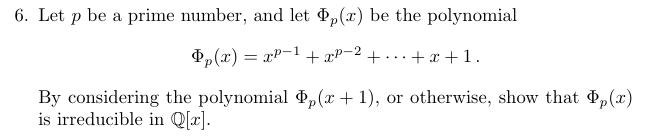
\includegraphics[scale=0.8]{6.png}
	\hfill
\end{problem}

\begin{solution}
We show that $\Phi(x)$ is irreducible using Eisenstein's criterion.

First we note that $\Phi(x+1)$ is irreducible over $\Q[x]$ if and only
if $\Phi(x)$ is irreducible over $\Q[x]$.
Suppose $\Phi(x+1)$ were reducible then write $\Phi(x+1) = f(x)g(x)$
for non-constant $f,g \in \Q[x]$. Now notice $\Phi(x) = f(x-1)g(x-1)$.
The substitution $x \mapsto x-1$ cannot make either $f,g$ constant
polynomials. And so we have have found a reduction of $\Phi(x)$. That
is, $\Phi(x+1)$ reducible implies $\Phi(x)$ is reducible. A similar
argument will give that $\Phi(x)$ reducible implies that $\Phi(x+1)$
is reducible. And so $\Phi(x)$ is reducible if and only if $\Phi(x+1)$
is reducible, all over $\Q[x]$. And so, we proceed by showing that
$\Phi(x+1)$ is irreducible over $\Q[x]$.

Next, notice that $\Phi(x) = \frac{x^p-1}{x-1}$. This can be shown by
multiplying out $\Phi(x)(x-1)$, we end up with telescoping terms and
the result is $x^p - 1$. 

It then follows that $\Phi(x+1) = \frac{(x+1)^p - 1}{x}$. Now, using
the binomial theorem, we have \[
(x+1)^p = x^p + \binom{p}{p-1}x^{p-1} + \cdots + \binom{p}{3}x^3 +
\binom{p}{2}x^2 + \binom{p}{1} x + 1.
\]
And so \[
	\frac{(x+1)^p - 1}{x}
	= x^{p-1} + \binom{p}{p-1} x^{p-2} + \cdots + \binom{p}{1}.
\]

We claim that this form allows us to deduce that the Eisenstein
criterion is fulfilled.
First, we have $a_n = 1$ and so $a_n$ is not in any prime ideal.
Moreover, we have that $\binom{p}{1} = p \not\in (p)^2 = (p^2)$ in
$\Z[x]$, but $p \in (p)$. 

Then lastly, we need to show that $\binom{p}{k} \in (p)$ for each $1 <
k < p$. Considering the algebraic formulation of the binomial
coefficient, we have, for each $k < n$ \[
	\binom{p}{k} = \frac{p!}{k!(p-k)!}.
\]
Notice that $p$ divides the numerator, but not the denominator.
Indeed, $k < n$ implies each factor of $k!$ is less than $p$, and so
$p$ does not divide $k!$. Similar reasoning gives that $p$ does not
divide $(p - k)!$. Moreover, the right hand side of the above equation
is an integer. There is no common factors of $p$ between the numerator
and denominator, and $p$ is prime, so by considering the prime
factorization of the right hand side, we have that $p$ divides $\binom{p}{k}$.
Eisenstein's irreducibility criterion is fulfilled and so $\Phi(x)$ is
irreducible over $\Q[x]$. 

\end{solution}

\newpage

%------------------------- Problem 7 -----------------------

\begin{problem}
	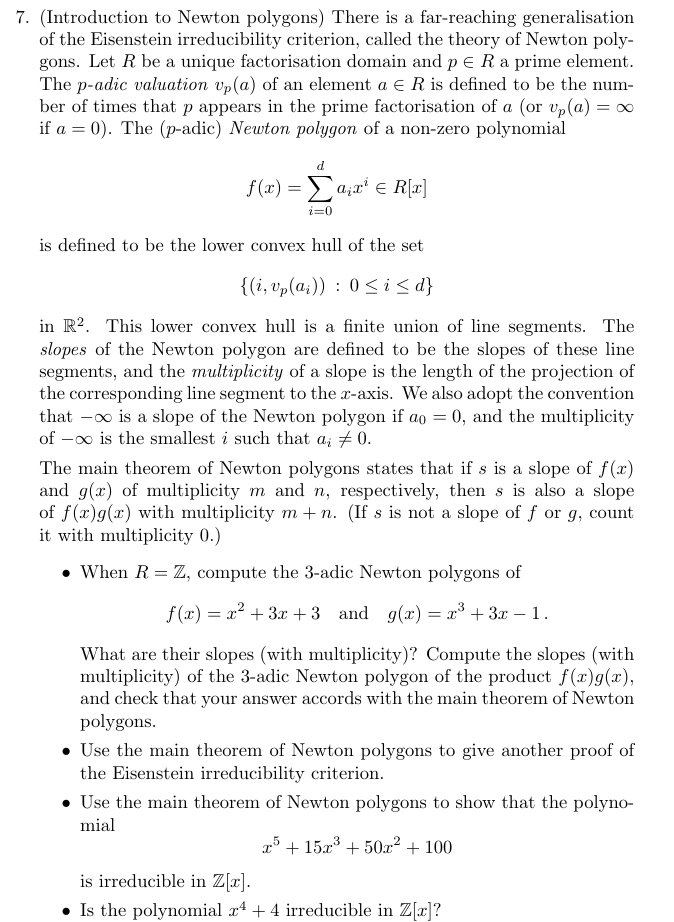
\includegraphics[scale=0.8]{7.png}
	\hfill
\end{problem}

\begin{solution}
\begin{itemize}
\item See Figure $(\ref{newt_a})$.
\begin{figure}[h]
	\centering
	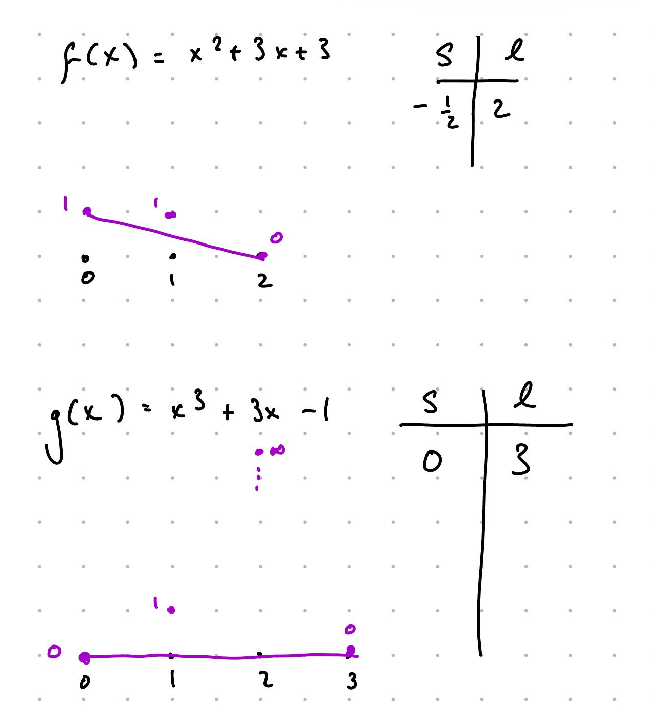
\includegraphics[scale=0.5]{newt_a.png}	
	\caption{$3$-adic newton polytopes for $f,g$ with slope data.
	The points are labelled with their $3$-adic valuation.}
	\label{newt_a}
\end{figure}

\item Recall the statement for Eisenstein's irreducibility criterion:
suppose $f(x) = \sum_{i=0}^{n} a_i x^i \in \Z[x]$ with, for some prime
$p$, $a_i \in (p)$ for $0 \geq i < n$, $a_0 \not\in (p^2)$, and $a_n
\not \in (p)$, then we have that $f$ is irreducible over $\mathbb Q
[x]$. If we additionally suppose that $f$ is primitive, then in fact
$f$ is irreducible over $\Z[x]$.

We use the main theorem of $p$-adic newton polygons to prove this
statment. Considering the $p$-adic newton polygon of the above
conditions gives us that $\nu_p(a_0) = 1$, $\nu_p(a_i) \geq 1$ for
each $i < n$, and $\nu_p(a_n) = 0$. This means we have slope data
$(-1/n, n)$ for $f$. Suppose, for contradiction, that $f$ is primitive and reducible. That
is we have some non-constant $g,h \in \Z[x]$ such that $h = fg$. 

Note that since $\nu_p(a_0(f)) = 1$ we must have that either $h$ or
$g$ has exactly one factor of $p$ in its constant term. Suppose,
without loss of generality, that $\nu_p(a_0(h)) = 1$. Then the only
way for the $p$-adic newton polytope of $f$ to have a slope of $-1/n$
is for $deg(f) = n$ and for $\nu_p(a_i(h)) \geq 1$ for each $i < n$
and for $\nu_p(a_n(h)) = 0$. Then, by the main theorem of newton
polytopes, we must have $deg(g) = 0$, a contradiction.

We also cannot have the case where $g$ is a constant, since we assumed
$f$ is primitive. It follows then that $f$ is irreducible over
$\Z[x]$. If $f$ were not primitive, we could divide its coefficients
by their greatest common divisor, and then the same argument would
give that $f$ is irreducible over $\Q[x]$. 

\begin{figure}[h]
	\centering
	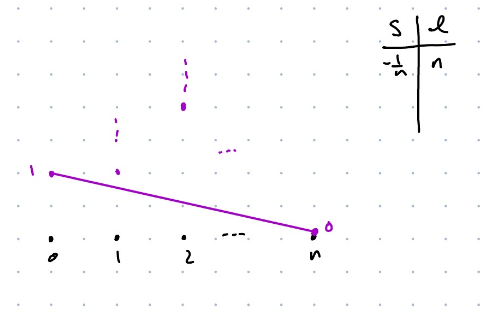
\includegraphics[scale=0.5]{newt_eisen.png}	
	\caption{The $p$-adic newton polytope given by the condition of
	Eisenstein's criterion.}
	\label{newt_eisen}
\end{figure}

\item We show that $h(x) = x^5 + 15x^3 + 50x^2 + 100$ is irreducible
over $\Z[x]$. Consider the slope data for the $5$-adic newton polytope
for $h$, we have $(-1/2, 5)$
\begin{figure}[h]
	\centering
	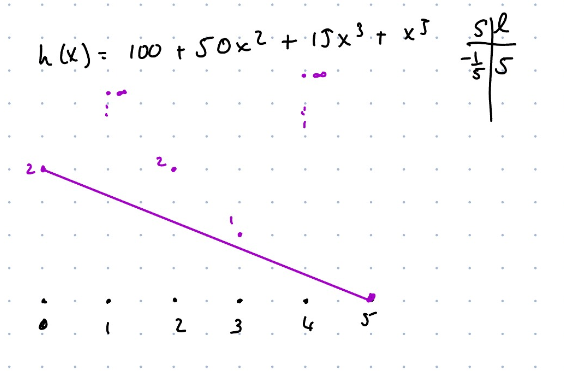
\includegraphics[scale=0.5]{newt_c.png}	
	\caption{The $5$-adic newton polytope with valuations of $h(x) = x^5 + 15x^3 + 50x^2 + 100$}
\end{figure}

Now suppose $h = fg$ for non-constant $f,g \in \Z[x]$.
Without loss of generality, we have two cases: either $def(f) = 1$ and $deg(g) = 4$ or $deg(f) =
2$ and $deg(g) = 3$.

First consider $deg(f) = 1$ and $deg(g) = 4$. Consider the $5$-adic
newton polytope for $f$. Since $f$ is degree $1$ we can only have
integer slopes in the $p$-adic newton polytope for $f$, for any $p$. 
And so, by the main theorem for $p$-adic newton polytopes, it's
impossible to choose coefficients for $f$ which is consistent with the
slope data for $h$.

Likewise, if we instead have $deg(f) = 2, deg(g) = 3$ then we have a
similar parity issue for the slopes of the $5$-adic newton polytope
for $g$. We know that $a_n(f) = a_n(g) = 1$ and so in particular
$\nu_5(a_n(g)) = 0$. Hence to have a slope of $-1/2$ we must have
$\nu_5(a_1(g)) = 1$ and $\nu_5(a_1(g)) \geq 1$. However, from here it
is impossible to choose coefficients for $a_0$ which gives us another
slope of length $-1/2$. Intuitively, there is ``not enough room''
for all the slopes to be $-1/2$ in the $5$-adic newton polytope for
$g$.

Lastly, since $h$ is monic there is no constant term which divides all
the coefficients of $h,f,g$. And so we cannot decompose $h$ into a
product of a non-unit constant and a degree $5$ polynomial.

All cases lead us to contradiction, and so it must be that one of
$f,g$ is a unit, and so $h$ is irreducible. 


\item Let $h(x) = x^4 + 4$ and consider the $2$-adic Newton Polytope
of $h$.
\begin{figure}[h]
	\centering
	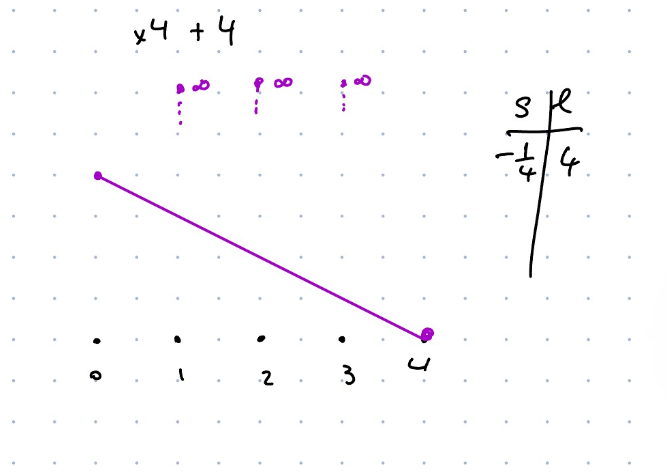
\includegraphics[scale=0.5]{newt_d.png}	
	\caption{Yet another $2$-adic newton polytope.
	NOTE: the slope, length data is incorrect in the image, we
	actually have $(-1/2, 4)$.
	}
\end{figure}
We claim that $h$ is reducible over $\Z[x]$. 
I already did all the work reasoning about the newton polytope data of
the factors, and so I will reproduce that here.
Write $h = fg$ where $f,g
\in Z[x]$. Notice that $h$ is primitive (since it is monic), so we can consider $f,g$
non-constant. We have two cases: either $deg(f) = 1, deg(g) = 3$ or
$deg(f) = deg(g) = 2$. In either case we must have the leading terms
for $f,g$ are $1$ and so $\nu_2(a_n) = 0$ for both $f,g$. 
Moreover, the constant terms for $f,g$ are either $\pm 1,
\pm 4$ or $\pm 2, \pm 2$.

Suppose first that $deg(f) = 1, deg(g) = 3$. 
Since $\nu_2(a_n(f)) = 0$, there is no possible
valuation $\nu_2(a_0(f))$ which will give us a slope of $-1/2$ for the
$2$-adic newton polytope of $f$. And so, by the main theorem of newton
polytopes, this case is not possible.

Suppose instead then that we have $\deg(f) = deg(g) = 2$. We have
$\nu_2(a_n(f)) = \nu_2(a_n(g)) = 2$ and so, to have $2$-adic newton
polytopes for $f,g$ which are consistent with $h$, we must have
$\nu_2(a_0(f)) = \nu_2(a_0(g)) = 2$. That is we have $a_0(f) = a_0(g)
= \pm 2$. And we must also have the degree $1$ terms for $f,g$ are
even, more precisely, $\nu_2(a_1(f)), \nu_2(a_1(g)) \geq 1$. 
Let us write $f(x) = 2 + ax + x^2$ and $g(x) = 2 + bx + x^2$.
Considering the coefficients of $f\cdot g$ gives us the following
system of equations 
\begin{align*}
	a &= -b \\
	b^2 &= 4.
\end{align*}
which has solutions in $\Z$: $a = 2$ and $b = -2$. Then, indeed \[
	(2 + 2x + x^2)(2 - x + x^2) = 4 + x^4.
\]
	Notice that these polynomials are primitive, and so are
	irreducible over $\Z[x]$.

\wg{
Note to self: 
This question was a saga for me, and despite the embaressement of getting the newton
polytope wrong initially, and spending so long on this question
I feel like I learned so much and have truly
ascended. What a delightful experience.
}

\end{itemize}
\end{solution}

\newpage



\end{document}
